\documentclass{article}
\usepackage{fullpage}

%load needed packages
\usepackage{graphicx}
\usepackage{array}
\usepackage{booktabs}
\usepackage[utf8]{inputenc}
\usepackage[T1]{fontenc}
\usepackage{url}
\usepackage[spanish]{babel} % Paquete para el idioma español
\usepackage{float}  % Necesario para [H]
\usepackage{listings}
\usepackage{xcolor}

\definecolor{codegreen}{HTML}{5AB2FF}
\definecolor{morado}{HTML}{AD88C6}
\definecolor{BG}{HTML}{EEEEEE}
\definecolor{azul}{HTML}{4D869C}
\definecolor{sqlblue}{HTML}{FF8C00} % Color para las palabras clave SQL

% Estilo para DDL
\lstdefinestyle{ddlstyle}{
	language=SQL,
	backgroundcolor=\color{BG},
	commentstyle=\color{codegreen},
	basicstyle=\ttfamily\small,
	keywordstyle=\color{azul},
	stringstyle=\color{morado},
	showstringspaces=false,
	breaklines=true,
	frame=shadowbox,
	numbers=left,
	numberstyle=\tiny\color{gray},
	captionpos=b,
}

% Estilo para SQL
\lstdefinestyle{sqlstyle}{
	language=SQL,
	backgroundcolor=\color{BG},
	commentstyle=\color{codegreen},
	basicstyle=\ttfamily\small,
	keywordstyle=\color{sqlblue}, % Color diferente para palabras clave SQL
	stringstyle=\color{morado},
	showstringspaces=false,
	breaklines=true,
	frame=shadowbox,
	numbers=left,
	numberstyle=\tiny\color{gray},
	captionpos=b,
}

\begin{document}



% Portada
\begin{titlepage}
	\centering
	\vspace*{3cm}
	
	% Título destacado
	{\Huge \textbf{Estracción, Transformación y Carga de datos en Almacén de Gasto en Medicamento}\\[0.5cm]}
	
	% Espacio y logotipo (si lo tienes, por ejemplo el logo de tu universidad)
	\vspace{2cm}
	
\includegraphics[width=0.3\textwidth]{images/uma_logo.jpg}\\[1cm]
	
	% Nombre del autor
	{\LARGE \textbf{Alejandro Silva Rodríguez}\\[0.5cm]}
	{\LARGE \textbf{Marta Cuevas Rodríguez}\\[0.5cm]}
	{\large \textit{Almacenes De Datos}\\
		Universidad de Málaga\\
		}
	
	\vfill
	
	% Fecha en la parte inferior de la página
	{\large Septiembre 2024}
\end{titlepage}

% indice
\tableofcontents

\newpage
\section{Introducción}
\label{sec:introduccion}

En el contexto hospitalario actual, el monitoreo y la gestión eficiente de los recursos es una necesidad apremiante, especialmente en unidades como la de Cuidados Intensivos (UCI), donde la administración de medicamentos representa una parte sustancial de los costos. A nivel mundial, el incremento en el costo de los medicamentos y la presión financiera sobre los sistemas de salud han impulsado la búsqueda de soluciones que optimicen el uso de los recursos en entornos críticos. Sin embargo, muchas instituciones hospitalarias carecen de herramientas analíticas específicas para monitorizar y analizar de manera detallada el gasto en fármacos, lo que limita la capacidad de identificar patrones de consumo y optimizar la asignación de presupuestos.\\

En el informe anterior se detalló el diseño e implementación de un almacén de datos diseñado para analizar el gasto en medicamentos en pacientes ingresados en la UCI en hospitales de EE.UU a partir de la base de datos proporcionada por el MIT \cite{eicu_crd}. Para abordar este desafío, el proceso de extracción, transformación y carga (ETL) se convierte en un componente clave, ya que permite integrar datos de diferentes fuentes, transformarlos en un formato homogéneo y almacenarlos en el almacén de datos. Este enfoque no solo facilita el análisis eficiente del gasto en medicamentos, sino que también garantiza la calidad y coherencia de los datos utilizados para la toma de decisiones.

\section{Objetivos}
\label{sec:objetivos}

El objetivo principal de este trabajo es implementar procesos de extracción, transformación y carga (ETL) para alimentar de manera eficiente dos almacenes de datos: el almacén NorthwindDW y un almacén diseñado para analizar el gasto en medicamentos en unidades de cuidados intensivos (UCI). Este propósito se concreta en los siguientes objetivos específicos:

\begin{itemize}
	\item Diseñar y ejecutar un proceso ETL completo para el almacén de datos NorthwindDW, utilizando herramientas y técnicas previamente estudiadas, con el fin de consolidar conocimientos y garantizar la correcta carga de todas sus tablas.
	\item Corregir el diseño del almacén de datos, de manera que facilite los procesos ETL.
	\item Implementar un proceso ETL personalizado para un almacén de datos orientado al análisis del gasto en medicamentos en las UCI.
	
\end{itemize}

\section{Almacén de Datos de NorthWind}

 El objetivo de esta parte del proyecto consiste en construir un almacén de datos (\texttt{NorthwindDW}) a partir de la base de datos \texttt{Northwind}. Para ello, se desarrolló un proceso de extracción, transformación y carga (ETL) que permite mover los datos desde la base de datos origen hacia el almacén, adaptándolos a su nueva estructura.

\subsection{Extracción, Transformación y Carga de Datos}

El flujo ETL diseñado se compone de múltiples tareas que se ejecutan de manera secuencial y/o paralela. Estas tareas incluyen la carga de diferentes dimensiones como \texttt{Employee}, \texttt{Category}, \texttt{Product}, entre otras, así como tablas relacionadas con jerarquías geográficas como \texttt{Continent}, \texttt{Country}, \texttt{State}, y \texttt{City}. Cada tarea se asegura de transformar los datos según las necesidades del almacén y garantizar su integridad y consistencia.
\\

En la Figura \ref{fig:NorthWind}, se presenta el flujo de control completo con todas las tareas ejecutadas satisfactoriamente. Este diagrama refleja el correcto funcionamiento del proceso ETL y el éxito en la carga de los datos.

\begin{figure}[H]
	\begin{center} 
		\includegraphics[width=0.65\textwidth]{images/cargaNorthwind.png} % Cambia 1 a 0.5 o el valor deseado
		\caption{Carga completa del almacén NorthwindDW}
		\label{fig:NorthWind}
	\end{center}
\end{figure}

Durante la implementación del proceso ETL (Extract, Transform, Load), se encontraron ciertas dificultades. Una de ellas ocurrió durante la carga de la tabla \texttt{Employee}. Al intentar insertar datos, surgió el siguiente error relacionado con restricciones de claves foráneas:

\begin{verbatim}
	[Empleado DW [68]] Error: An exception has occurred during 
	data insertion, the message returned from the provider is: 
	Se terminó la instrucción. Instrucción INSERT en conflicto 
	con la restricción FOREIGN KEY SAME TABLE 'FK_Employee_Employee'. 
	El conflicto ha aparecido en la base de datos 'NorthwindDW', 
	tabla 'dbo.Employee', column 'EmployeeKey'.
\end{verbatim}

Este problema se debía a que la tabla \texttt{Employee} contenía una clave foránea que referenciaba a sí misma, lo cual generaba conflictos al insertar los datos en un orden incorrecto. Para resolverlo, se deshabilitaron temporalmente las restricciones de claves foráneas antes de la carga de datos mediante el comando SQL:

\begin{verbatim}
	EXEC sp_MSForEachTable 'ALTER TABLE ? NOCHECK CONSTRAINT ALL';
\end{verbatim}

Una vez finalizada la carga de datos, se volvieron a habilitar las restricciones para asegurar la integridad referencial del almacén con el siguiente comando:

\begin{verbatim}
	EXEC sp_MSForEachTable 'ALTER TABLE ? WITH CHECK CHECK CONSTRAINT ALL';
\end{verbatim}

Gracias a esta solución, el proceso de carga se completó exitosamente. 

\section{Almacén de Datos de Gasto de Medicamento en UCI}

\subsection{Rediseño del Almacén}

Antes de proceder con el llenado del almacén, se realizó un rediseño significativo de su estructura para optimizar su funcionamiento y facilitar la integración con la base de datos de origen. 
\begin{figure}[H]
	\begin{center} 
		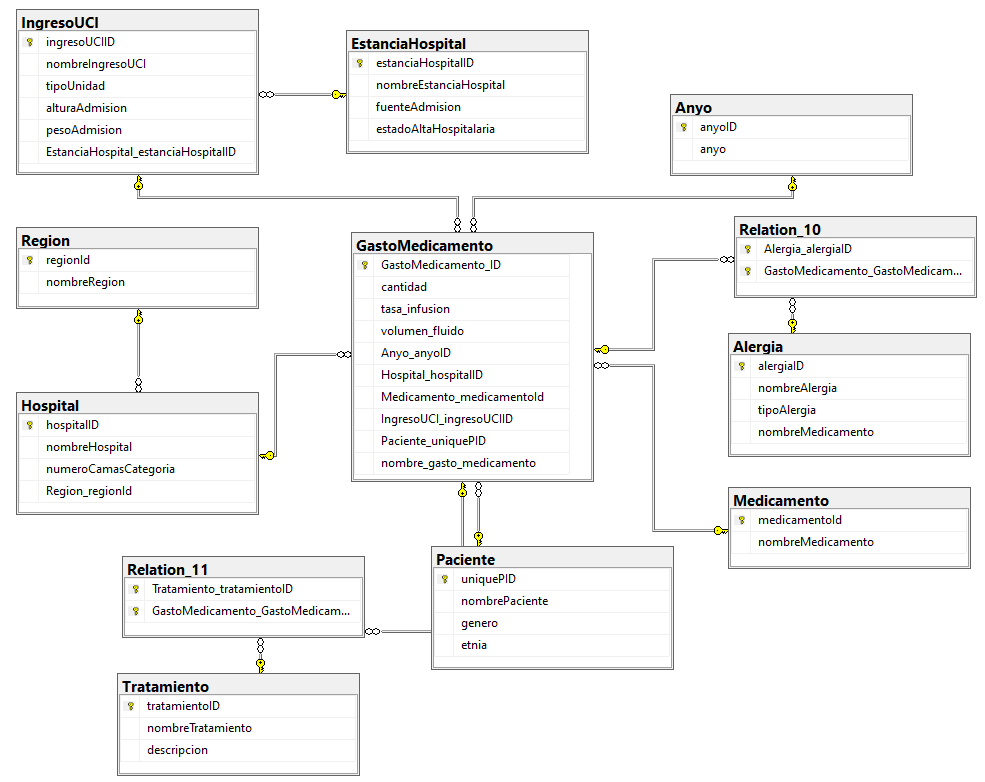
\includegraphics[width=0.65\textwidth]{images/nuevo_diseno.png} % Cambia 1 a 0.5 o el valor deseado
		\caption{Rediseño del almacén para gastos en medicamentos}
		\label{fig:nuevo_diseño}
	\end{center}
\end{figure}
Como se puede observar en la Figura \ref{fig:nuevo_diseño}, este rediseño incluye varios cambios clave:

\begin{itemize}
	\item \textbf{Autogeneración de identificadores (IDs):} En el nuevo diseño, los identificadores principales de las tablas ahora son generados automáticamente por el sistema, en lugar de depender de los valores provenientes de la base de datos de origen. Esto asegura consistencia y evita problemas de duplicados.
	
	\item \textbf{Preservación de IDs originales como atributos:} Los identificadores originales de la base de datos de origen se han mantenido, pero ahora figuran como atributos adicionales en las clases correspondientes codificadas como "nombre[clase]" .Esto permite rastrear fácilmente el origen de los datos y establecer vínculos con sistemas externos cuando sea necesario.
	
	\item \textbf{Adición de nuevos atributos:} Se han incorporado más atributos en algunas tablas para enriquecer la información almacenada. Por ejemplo:
	\begin{itemize}
		\item En la tabla \texttt{Paciente}, se han añadido atributos como el género y la etnia.
		\item La tabla \texttt{EstanciaHospital} incluye ahora información sobre la fuente de admisión y el estado al alta hospitalaria.
		\item La tabla \texttt{GastoMedicamento} incluye atributos como el volumen de fluido y el tipo de infusión.
	\end{itemize}
\end{itemize}

Estos cambios no solo mejoran la estructura y la claridad del diseño del almacén, sino que también amplían su capacidad para almacenar información detallada, facilitando futuros análisis y consultas complejas.


\subsection{Creación de un Nuevo Proyecto en SQL Server Management Studio}

A continuación, se describe el proceso para crear un nuevo proyecto en SQL Server Management Studio (SSMS), paso a paso:

\paragraph{Paso 1: Abrir SQL Server Management Studio}  
Abre SQL Server Management Studio desde el menú de inicio de tu sistema operativo. Si no lo tienes instalado, puedes descargarlo desde el sitio oficial de Microsoft.

\paragraph{Paso 2: Iniciar un Nuevo Proyecto}  
Sigue los pasos a continuación para crear un nuevo proyecto en SSMS:
\begin{enumerate}
	\item En el menú principal de SSMS, haz clic en \textbf{Archivo} (\textit{File}).
	\item Selecciona \textbf{Nuevo Proyecto} (\textit{New Project}).
	\item En la ventana emergente, selecciona el tipo de proyecto llamado \textbf{Proyecto de Base de Datos} (\textit{Database Project}). Este tipo de proyecto te permite gestionar el desarrollo de bases de datos de manera organizada.
	\item Asigna un nombre a tu proyecto en el campo \textbf{Nombre del Proyecto} (\textit{Project Name}), como por ejemplo: \texttt{BorradoAlmacenProyecto}.
	\item Elige una ubicación para guardar tu proyecto en el campo \textbf{Ubicación} (\textit{Location}). Asegúrate de seleccionar una carpeta fácil de localizar.
	\item Si es necesario, selecciona también un \textbf{Nombre de Solución} (\textit{Solution Name}). Esto es útil si planeas agrupar varios proyectos relacionados.
	\item Haz clic en \textbf{Aceptar} (\textit{OK}) para crear el proyecto.
\end{enumerate}

\paragraph{Paso 3: Configurar Conexión a la Base de Datos}  
Una vez creado el proyecto:
\begin{enumerate}
	\item En la barra de herramientas de SSMS, haz clic en \textbf{Ver} (\textit{View}) y selecciona \textbf{Explorador de Objetos} (\textit{Object Explorer}).
	\item En el panel de \textit{Object Explorer}, haz clic derecho sobre \textbf{Conexiones de Servidor} (\textit{Server Connections}) y selecciona \textbf{Conectar} (\textit{Connect}).
	\item Introduce los detalles de conexión a tu servidor SQL, como:
	\begin{itemize}
		\item Nombre del servidor (\textit{Server Name}): Por ejemplo, \texttt{localhost} o el nombre de tu servidor.
		\item Tipo de autenticación (\textit{Authentication}): Selecciona \texttt{Windows Authentication} o \texttt{SQL Server Authentication} según corresponda.
	\end{itemize}
	\item Haz clic en \textbf{Conectar} (\textit{Connect}) para enlazar el proyecto con la base de datos deseada.
\end{enumerate}


\subsection{Extracción, Transformación y Carga de Datos}

\subsection{Borrado del Almacén}

Para realizar el borrado completo del almacén de datos, es necesario crear un procedimiento almacenado en SQL Server Management Studio (SSMS). Esto se lleva a cabo en el almacén de datos vacío llamado \texttt{NorthwindDW}, accediendo a la sección \texttt{Programmability} y creando un nuevo \texttt{Stored Procedure}. 

El procedimiento debe incluir las instrucciones necesarias para eliminar los datos de las tablas en el orden correcto, comenzando por las tablas que tienen dependencias externas (o relaciones con otras tablas) y finalizando con aquellas más internas (las que no tienen dependencias hacia otras tablas). Esto asegura que las restricciones de claves foráneas no causen errores durante el proceso de eliminación.

\begin{lstlisting}[style=ddlstyle, label=fig:borradoAlmacen,caption=Borrado del Almacen de UCI]
	USE UCIDW;
	GO
	
	SET ANSI_NULLS ON;
	GO
	SET QUOTED_IDENTIFIER ON;
	GO
	
	CREATE OR ALTER PROCEDURE BorrarAlmacen	
	AS
	BEGIN
	BEGIN TRY
	-- Iniciar transaccion
	BEGIN TRANSACTION;
	
	-- Eliminar datos de las tablas
	
	DELETE FROM Relation_10;
	DELETE FROM Relation_11;
	
	DELETE FROM GastoMedicamento;
	
	
	DELETE FROM Medicamento;
	DELETE FROM Alergia;
	DELETE FROM Anyo;
	DELETE FROM Tratamiento;
	
	DELETE FROM Hospital;
	DELETE FROM Region;
	
	DELETE FROM IngresoUCI;
	DELETE FROM EstanciaHospital;
	
	DELETE FROM Paciente;
	
	
	
	-- Reiniciar los valores de identidad
	DBCC CHECKIDENT ('Medicamento', RESEED, 0);
	DBCC CHECKIDENT ('Alergia', RESEED, 0);
	
	DBCC CHECKIDENT ('Tratamiento', RESEED, 0);
	DBCC CHECKIDENT ('Region', RESEED, 0);
	DBCC CHECKIDENT ('Hospital', RESEED, 0);
	DBCC CHECKIDENT ('EstanciaHospital', RESEED, 0);
	DBCC CHECKIDENT ('IngresoUCI', RESEED, 0);
	DBCC CHECKIDENT ('Paciente', RESEED, 0);
	
	DBCC CHECKIDENT ('GastoMedicamento', RESEED, 0);
	
	-- Confirmar transaccion
	COMMIT TRANSACTION;
	END TRY
	BEGIN CATCH
	-- Deshacer transaccion si ocurre un error
	IF @@TRANCOUNT > 0
	ROLLBACK TRANSACTION;
	
	-- Rethrow del error para depuracion
	THROW;
	END CATCH;
	END;
	GO
\end{lstlisting}


En el \texttt{Listing \ref{fig:borradoAlmacen}}, se describe el contenido del procedimiento almacenado \texttt{BorrarAlmacen}, que realiza las siguientes operaciones clave:

\begin{enumerate}
	\item \textbf{Inicio de una transacción:} Se utiliza \texttt{BEGIN TRANSACTION} para garantizar que todas las operaciones de eliminación se realicen de forma atómica. En caso de que ocurra un error, la transacción puede revertirse completamente mediante \texttt{ROLLBACK TRANSACTION}.
	
	\item \textbf{Eliminación de datos:} Los datos se eliminan de todas las tablas, siguiendo el orden correcto:
	\begin{itemize}
		\item Se empieza eliminando las relaciones secundarias (\texttt{Relation\_10} y \texttt{Relation\_11}).
		\item Posteriormente, se eliminan las tablas principales como \texttt{GastoMedicamento}, \texttt{Medicamento}, \texttt{Alergia}, \texttt{Anyo}, \texttt{Tratamiento}, \texttt{Hospital}, \texttt{Region}, \texttt{IngresoUCI}, \texttt{EstanciaHospital} y \texttt{Paciente}.
	\end{itemize}
	
	\item \textbf{Reinicio de valores de identidad:} Después de eliminar los datos, se reinician los valores de identidad en las tablas afectadas usando el comando \texttt{DBCC CHECKIDENT}. Esto asegura que los identificadores autogenerados comiencen desde cero para futuras inserciones.
	
	\item \textbf{Confirmación de la transacción:} Una vez completadas todas las eliminaciones y reinicios, la transacción se confirma mediante \texttt{COMMIT TRANSACTION}.
	
	\item \textbf{Gestión de errores:} En caso de un error, el bloque \texttt{CATCH} revierte la transacción para preservar la integridad del almacén de datos y re-lanza la excepción con el comando \texttt{THROW}, facilitando la depuración.
\end{enumerate}

Este procedimiento asegura que el almacén de datos esté completamente vacío y listo para ser llenado nuevamente, mientras se mantiene la consistencia y se manejan posibles errores durante el proceso.

\subsubsection{Integración del Eliminado de alamcén en SQL Server Management Studio (SSMS)}



\begin{figure}[H]
	\begin{center} 
		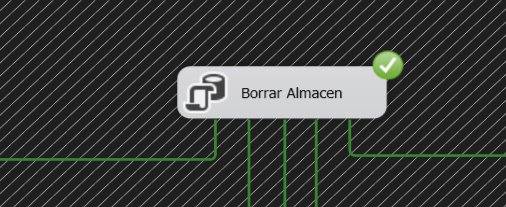
\includegraphics[width=0.65\textwidth]{images/completados/borrado_almacen.png} % Cambia 1 a 0.5 o el valor deseado
		\caption{Carga completa del borrado del almacén}
		\label{fig:borrado_completo}
	\end{center}
\end{figure}

\section{Dificultades Encontradas}
\label{sec:dificultades_encontradas}

A lo largo del proyecto nos hemos encontrado con varios obstáculos que nos han hecho replantear algunos aspectos del diseño del almacén de datos para la gestión hospitalaria:

\begin{enumerate}
	\item \textbf{}:
\end{enumerate}

A pesar de estas dificultades, cada uno de estos retos nos ha ayudado a entender mejor las particularidades del sector salud y a preparar un diseño más sólido para el almacén de datos.

\section{Conclusión}
\label{sec:conclusion}

Gracias a la organización del almacén de datos, se optimiza la consulta de información relevante para la toma de decisiones, facilitando la identificación de patrones de gasto asociados a diversas variables, como tratamientos específicos o características de los pacientes. Esta estructura, además, sienta las bases para futuras ampliaciones o análisis más complejos, promoviendo la escalabilidad y adaptabilidad del sistema. En conclusión, el proyecto aporta un modelo sólido y adaptable para la gestión y análisis de datos en el ámbito hospitalario, contribuyendo a una administración más eficiente de los recursos y a una mejora potencial en la atención a los pacientes.

\newpage
\section{Acceso al Repositorio}

Toda la información adicional, incluyendo el código fuente y la documentación completa de este proyecto, está disponible en el repositorio de GitHub \cite{silva2024github}.

% Incluir la bibliografía
\bibliographystyle{plain}  % Estilo de la bibliografía (por ejemplo, plain, alpha, ieee, etc.)
\bibliography{bibli}  % Nombre del archivo .bib sin la extensión

\end{document}
